\section{Methodology}
\label{sec:method}

Our main goal is to create a robust video surveillance road traffic monitoring system able to track vehicles, count them and estimate their speed, raising an alarm if any of them exceeds the speed limit established for the road.\\

\noindent Our system is based entirely on motion, and its complete pipeline is described in Fig. \ref{fig:pipeline}. The first step, in case the sequence is jittery, is to perform video stabilization using Target Tracking. Then, the foreground is segmented using Stauffer \& Grimson algorithm \cite{stauffer1999adaptive}, and morphological operations are applied to improve the segmentation. Once a series of blobs have been detected on each frame, a Kalman Filter is used to track them along the video sequence. Finally, using some knowledge of the scene geometry, the vehicles are counted and their speeds are estimated, raising an alarm if any of them exceeds the ---known--- limit.

\begin{figure}[htb]
\centering
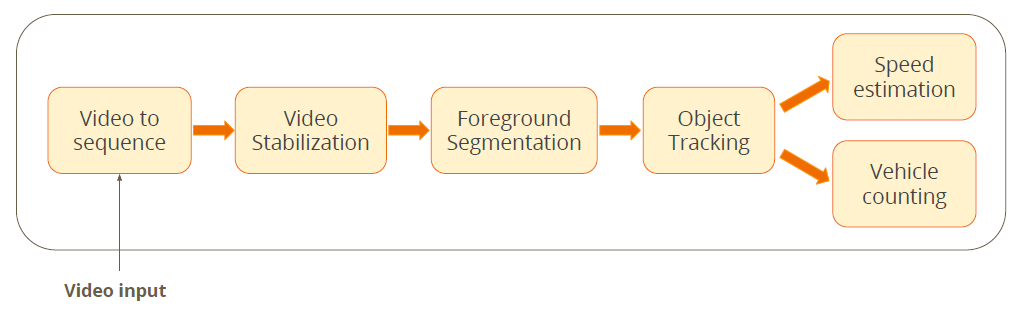
\includegraphics[width=0.9\linewidth, height = 3cm]{figures/pipeline}
\caption{Video Surveillance for Road Traffic Monitoring System pipeline.}
\label{fig:pipeline}
\end{figure}

\noindent The whole system has been implemented in Matlab, and the code is available at our Github repository \footnote{\url{https://github.com/mcv-m4-video/mcv-m4-2017-team2}}.

\subsection{Target Tracking Video Stabilization}
\label{sec:stabilization}
Video stabilization is a family of techniques used to reduce blurring associated with the motion of the camera  during exposure, and it generally compensates for pan and tilt of the camera, although rotations can also be compensated.\\

\noindent The main idea of Target Tracking Video Stabilization \footnote{\url{https://es.mathworks.com/help/vision/examples/video-stabilization.html}} is to use a block-based parametric motion model to correct translational and rotational camera motions. We define the target to track (in our system a square area in the lower left corner) and we establish a dynamic search region, whose position is determined by the last known target location. Then, we search for the target only within this search region. In each subsequent video frame we determine how much the target has moved relative to the previous frame, and we use this information to remove unwanted translational camera motions and generate a stabilized video. Notice that we add a black padding to all the frames to deal with the loss of information in the borders after stabilization, and we apply the same stabilization and padding to the ground truth for evaluation.

\begin{figure}[h]
\centering
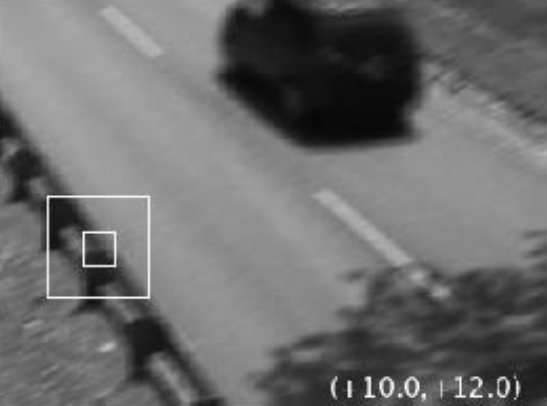
\includegraphics[width=105pt, height=95pt]{figures/target_tracking.png} 
\caption{Target Tracking Video Stabilization frame. The square on the left bottom area denotes the area to track used by the stabilization algorithm.}
\label{fig:fg}
\end{figure}
\subsection{Background Subtraction \& Foreground Detection}
\label{sec:bg_fg}
Both background and foreground are modeled using Gaussian Mixture Models (GMM), as proposed by Stauffer and Grimson \cite{stauffer1999adaptive}, a reliable technique that offers robustness against lighting changes, repetitive motions and long-term changes in the scene. It is based on the temporal observation of the pixels, and several Gaussians are used to represent either foreground or background. Gaussians are considered as background if they have high weight and low variance, and as foreground if they have low weight and high variance, and a pixel is assigned as background or foreground depending on its nearest Gaussian. \\

\noindent Once a foreground segmentation has been obtained, morphological operators are applied to improve the binary mask. First, closing and opening operators are applied to get better defined blobs. Then, a filling holes algorithm is used to avoid holes in the blobs. And last, an area filtering is used to remove the possible noise. Fig. \ref{fig:fg} shows an example of foreground detection for a frame of the highway sequence. 

\begin{figure}[h]
\centering
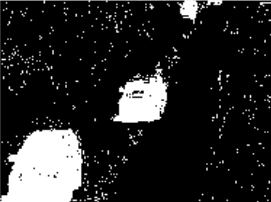
\includegraphics[width=85pt, height=75pt]{figures/fg_mask.png} 
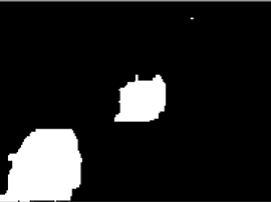
\includegraphics[width=85pt, height=75pt]{figures/fg_mask_mo.png} 
\caption{Foreground segmentation. On the left, the mask obtained with S\&G. On the right, the same mask after applying morphological operators.}
\label{fig:fg}
\end{figure}


\subsection{Tracking Vehicles}
\label{sec:tracking}

In order to achieve the goals of the system, vehicle counting and speed estimation, it is necessary to keep track of the vehicles in the scene. This means knowing how the detected blobs relate to each other between consecutive frames.\\

\noindent For this purpose, we assume a Linear Dynamics Model (LDM) and, consequently, a Kalman filter \cite{kalman} is used for tracking. Under this framework, the state of each vehicle is supposed to vary linearly on each time step and suffer a slight perturbation (with Gaussian distribution). Similarly, the detection obtained is supposed to be a linear transformation of the previous state, plus some Gaussian noise as well. The procedure consists of making a prediction of the object's next state, based on all the previous measurements, and once the new detection is done, update this prediction. The equations derived by the Kalman filter are the optimal ones in the case of an LDM.\\

\noindent The assumption of a linear model is not so restrictive as it may seem. This can handle, for instance, the projection (into the camera plane) of the movement of cars traveling at a constant speed. In almost any road it is possible to find sectors with this characteristics. A 50 meter long straight part of the road would be enough for our system to work. Fig. \ref{fig:kalman} shows an example of kalman tracking for 2 vehicle in our sequence.

\begin{figure}[h]
\centering
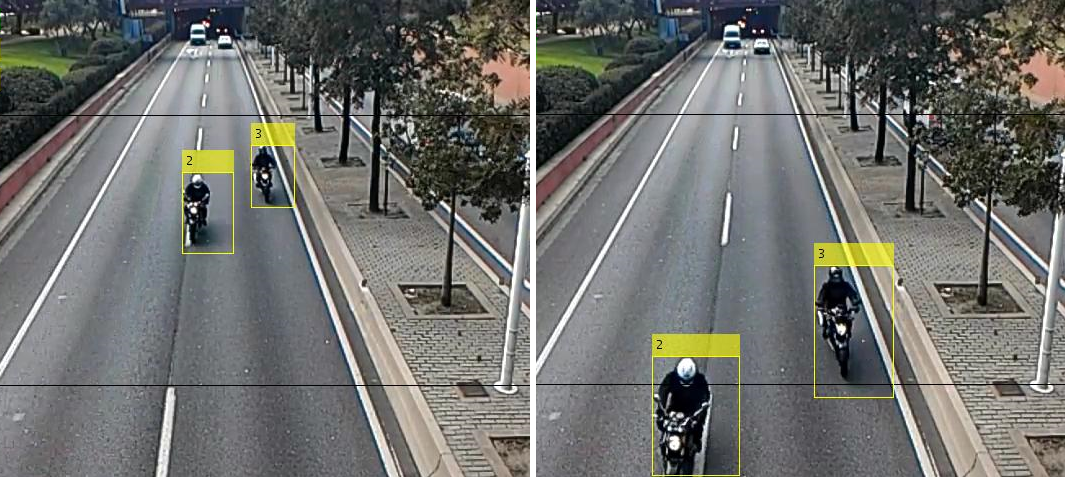
\includegraphics[width=240pt, height=130pt]{figures/example_kalman.png}
\caption{Sample of Kalman tracking detection for two vehicles along different frames.}
\label{fig:kalman}
\end{figure}
\subsection{Speed Estimator}
\label{sec:speed}
Our system provides an estimation on the speed of each tracked vehicle, rising a visual alarm when the speed limits are exceeded. Other works on this field make use of the optical flow in order to make motion estimations, but this approach requires the conversion of pixels/frame to distance/time. Even though it is a feasible task, prior knowledge of pixels/distance ratio in the sequence is mandatory. Moreover, perspective generates a progressive distortion in this ratio along the regions of the image, which can be mitigated by the use of homography techniques. The need for a controlled test with a vehicle for calibration stands as a major drawback.\\ 

\noindent To avoid the above-mentioned problems we came up with a more straightforward approach based on a single estimation per track, reference points in the view field, and a known distance. This method does not need much calibration to achieve good results, and it requires fewer resources making its implementation simpler. We set 2 reference lines as seen in Fig. \ref{fig:layout} in the road and we compute the frame difference between the vehicle crossing the first marker and reaching the second one. Knowing the frame rate of the video and the distance between markers, speed is calculated by a simple equation. \\

\noindent This method relies on the assumption that the tracked detection is precise and the bounding box is considered the vehicle itself. This avoids the use of the detection's centroid, which introduces greater distortion in the relative distance to the marker line than a border does. It is most desirable that the vanishing point lies out of frame for the perspective to be less distorting. This assumption approximates the real case scenario quite well provided that the distance between markers is as big as possible. The further away the markers are with respect to each other, the less influence a distance error will have on the estimated speed.

\begin{figure}[t]
\centering
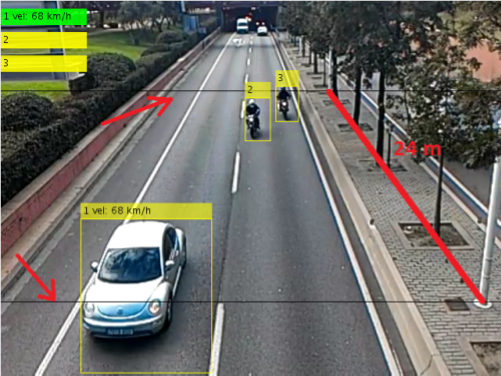
\includegraphics[width=0.9\linewidth]{figures/system}
\caption{System speed estimation layout with markers and distance pointed in red.}
\label{fig:layout}
\end{figure}

  





